\documentclass[a4paper]{article}
\usepackage{amsmath} %pour tous les trucs de math
\usepackage{systeme} %pour tous les systemes d'équations
%\usepackage{ bbold }  %pour toutes les doubles lettres
\usepackage{ dsfont } %pour le double 1
\usepackage{amssymb}  %pour les double Lettres
\usepackage{IEEEtrantools} %pour les équations en collonnes
\usepackage{amsthm} %pour les preuves
\usepackage[english]{babel} % la langue utilisée
\usepackage[utf8]{inputenc} % encodage symboles entrée
\usepackage[T1]{fontenc} % encodage symboles sortie
\usepackage{fancyhdr} %pour les entêtes et pied de page
%\usepackage[math]{blindtext} % pour le Lorem ipsum
%\usepackage{enumitem} %pour changer les listes
\usepackage[a4paper,textwidth=15cm,,textheight=25cm]{geometry}
%\usepackage[framed,numbered]{mcode} %MatLab
\usepackage{minted}
\usepackage{graphicx} % pour les graphiques
%\usepackage{subfig} % pour les doubles figures
\usepackage{float} % pour bien positionner les figures
\usepackage[dvipsnames]{xcolor} % pour la couleur du texte et de la page
%\usepackage{biblatex} % bibliographie
%\usepackage{csquotes} % pour que la biblio s'adapte à la langue
\usepackage{prettyref}
\usepackage[hidelinks]{hyperref} % pour les hyperliens et références(mettre en dernier)


\newrefformat{fig}{Figure~[\ref{#1}]}
\newrefformat{it}{question~\ref{#1}.}
\newrefformat{eq}{equation~(\ref{#1})}
\newrefformat{seq}{Section~\ref{#1}}
\newrefformat{th}{Theorem~\ref{#1}}
\newrefformat{lem}{Lemma~\ref{#1}}
\newrefformat{cor}{Corollary~\ref{#1}}
\newrefformat{rem}{Remark~\ref{#1}}

\newtheorem{theoreme}{Theorem} %[section]
\newtheorem{corollaire}{Corollary} %[theorem]
\newtheorem{lemme}{Lemma} %[theorem]
\theoremstyle{definition}
    \newtheorem{definition}{Definition} %[section]
\theoremstyle{remark}
     \newtheorem*{remarque}{Remark}

\pagestyle{fancy}
%\fancyhf{}
\lhead{Stochastic Simulations}
\chead{Autumn Semester 2021}
\rhead{Benoît Müller}

\title{Stochastic Simulations: Project 5 \\
\bf{QMC integration of non-smooth functions: application to pricing exotic options} }
\author{Benoît Müller}

\DeclareMathOperator*{\argmin}{argmin}
\DeclareMathOperator*{\argmax}{argmax}
\newcommand{\R}{\mathbb{R}}
\newcommand{\N}{\mathbb{N}}
\newcommand{\Z}{\mathbb{Z}}
\newcommand{\C}{\mathbb{C}}
\newcommand{\un}{\mathds{1}}
\newcommand{\s}{\sigma}
\newcommand{\starteq}{\begin{IEEEeqnarray*}{rCl}}
\newcommand{\stopeq}{\end{IEEEeqnarray*}}
\newcommand{\com}[1]{\textcolor{ForestGreen}{[~\emph{#1}~]}}
\newcommand{\python}[1]{\inputminted[linenos,frame=single]{python}{#1}}
\newcommand{\startpython}{\begin{minted}[linenos,frame=single]{python}}
\newcommand{\stoppython}{\end{minted}}
\chardef\_=`_ %pour l'underscore
%\newcommand{\nom}[nombre d’arguments]{définition(#1,#2,...,#n)}

\begin{document}
\maketitle
\part*{Preparations}
To re-cast the integral into a hypercube, we rewrite it first in terms of into uniform random variables in $[0,1]$. To do this we write the discretized Brownian motion in term of normal variables by Gaussian increments $\xi_i$:
$$w_{t_i} = w_{t_{i-1}}+\sqrt{t_i-t_{i-1}}\xi_i 
= \sum_{k=1}^i \sqrt{t_k-t_{k-1}}\xi_k \text{\quad for } i\in\{1,\dots,m\}$$
with $t_i=i T/m$ and $\xi_i$ some independent normal standard variables.
Now we write $\xi_i$ using uniform variables $U_i$. For efficiency and because we can impose the dimension to be even, we choose the Box-Müller method\footnote{I'm a Mister Müller too but I promise I don't receive any royalties on the spread of this fancy method.}:
$$
\xi_{2k,2k-1} = \sqrt{-2\log{U_{2k}}}(\cos,\sin)(2\pi U_{2k-1}) 
\text{\quad for } k\in\{1,\dots,m/2\} $$
We can write now explicitly $\Psi_i=\theta_i(U)\un_{\phi(U)}$ for a uniform variable $U$ in $\R^m$. We fix $m$ and define the functions related to the transformations: $ S_i=S_{t_i}$, $ Z_i(U)$ for the Gaussian variables , $W_i(Z)$ for the Brownian motion.
\starteq
\phi(U)
&=&\frac{1}{m}\sum_{i=1} ^m S_i\big(W_i(U)\big) - K\\
&=& \frac{1}{m}\sum_{i=1} ^m S_i\big(\sum_{k=1}^i  \sqrt{t_k-t_{k-1}}Z_k(U)\big) - K\\
&=& \frac{1}{m}\sum_{i=1} ^m S_0 e^{(r-\s^2/2)t_i + \s\sum_{k=1}^i \sqrt{t_k-t_{k-1}}Z_k(U)} - K \IEEEyesnumber \label{eq:trans} \\
&=& \frac{1}{m}\sum_{i=1} ^m S_0 e^{(r-\s^2/2)t_i + \s\sum_{k=1}^i \sqrt{t_k-t_{k-1}}Z_k(U)} - K
\stopeq
where we have fixed $m$

\part{}
%First estimate the value of the integral, as well as the error of the estimation, using a crude Monte Carlo and a randomized QMC, without the pre-integration trick, i.e., by generating (Q)MC sample $(z^{(1)},\dots, z^{(N)})$ over the $m$-dimensional unit cube ${[0, 1]}^m$. Try increasing values of the samples size $N = 27,\dots, 213$ and plot the estimated error versus $N$. Comment on the observed convergence rate.
We decide to go for an object-oriented implementation, using classes of objects. First, we will use along the project a upper class called \texttt{RandomVariable}, which contain general statistical purpose methods such as the confidence interval. It has a property $X$ for the random sample and N for its length.

We create now a subclass \texttt{Payoff} that define the random variable $\Psi$ for fixed parameters passed in properties: $m$, $K$, $S_0$, $r$, $\s$, $T$, and the time steps $(t_i)_i$. The methods will consist of the core of the code. We try to vectorize functions as we can, putting always the dimension $m$ in the last axis of the Numpy arrays.

We define then some methods for the variables $S(w)$, $\theta(w)$\com{il faudra changer le nom de theta en phi ici et dans le code}, $\Psi_i(w)$ for $i=1,2$, $Z(U)$, $W(Z)$, and they help us to define the two final transformations from $U$ to $\Psi_i$. From this, we write a random variable sample generator that return the transformation of a uniform random sample.

The Monte Carlo (MQ) method use \texttt{rvs} to generate $N$ samples and return the confidence interval. For the Quasi Monte Carlo (QMC) method, we use the module \texttt{SoboL\_new} given in the Lab \com{numero du lab}, that generate low discrepancy points sets, so we can try to see if this increase the order of the error. We then transform these points by \texttt{transform} and take the average on N of them. To randomize the method and compute an standard error, we repeat the process $k$ times while shifting all points by vector randomly generated with a uniform distribution. We choose $k$ fixed with value 20 so it does not cost too much more time. The precision of the mean was already qualitative with the $N$ sampling, and this is only for error estimation purposes.
\\ \\
We will see the evolution for different values of N, but we haven't vectorized the (Q)MC methods with respect to N, or build update formulas for the mean and variance. This doesn't affect the efficiency of the utilization of the (Q)MC methods but just our study of the error.

We fix the variables $K=S_0=100$ and $r=\s=0.1$ for now, and consider the dimension $m$ taking values in $\{2^5,\dots,2^{10}\}$ and compute for sample of lengths $N$ in $\{2^7,\dots,2^{14}\}$. We set the confidence as $1-\alpha=1-0.01$.
The plots we display show in a first time the evolution of the mean and its interval around in a log-scale for the x-axis which represent $N$ (\prettyref{fig:q1interval}):
\begin{figure}[H] 
    \centering{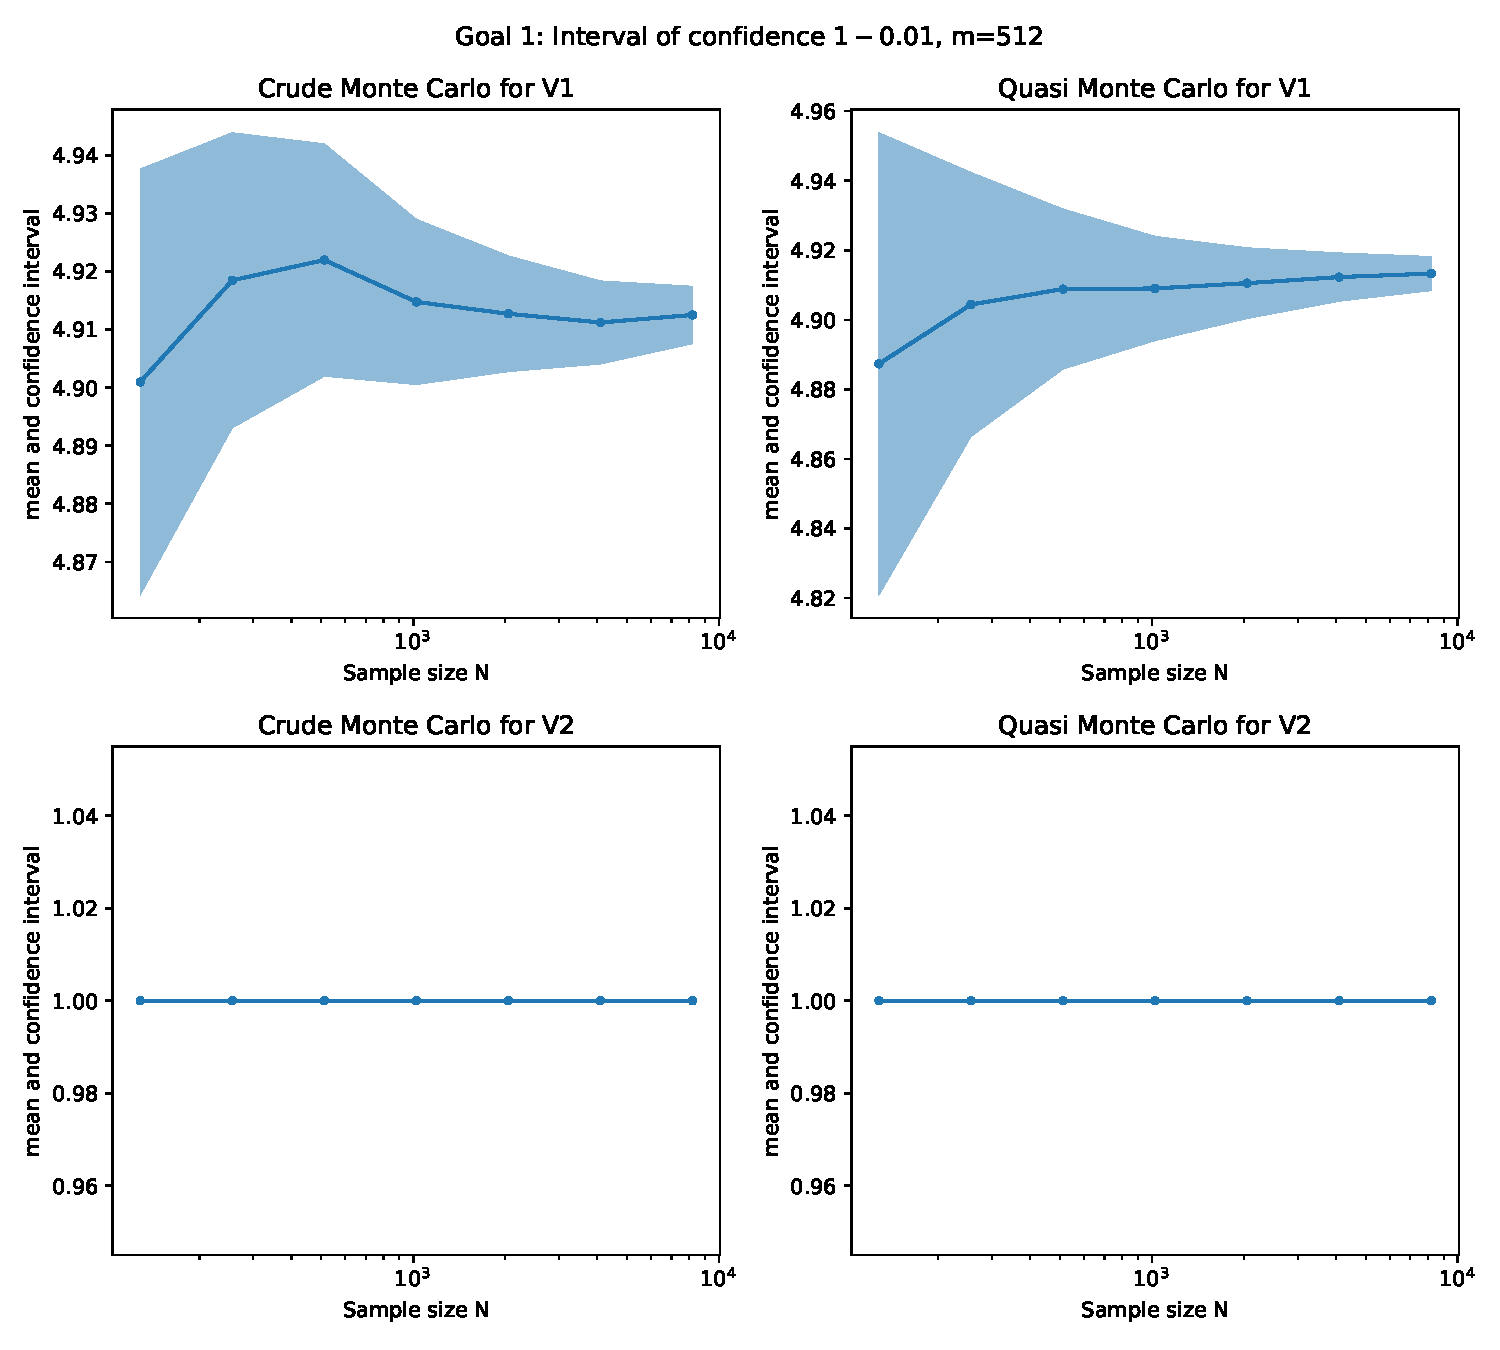
\includegraphics[width=\textwidth]{graphics/q1interval.pdf}}
    \caption{Evolution of the mean and the interval given by (Q)MC with respect to the sample size}
    \label{fig:q1interval}
\end{figure}
We see that both methods seem to converge to the same value. Even if the mean need time to be stabilized, all the intervals always contain the final mean done with the most precision and attest their coherence.
The output is:
\\\\
The computed intervals for m = 512 , N = 8192 and alpha = 0.1 are:\\
V1:  MC: 5.811725874367571 ± 0.09548596396958434\\
$\quad$ QMC: 5.817669062629391 ± 0.02093917604003062\\
V2:  MC: 0.799072265625 ± 0.007282353659082176\\
$\quad$   QMC: 0.797613525390625 ± 0.0016172925932021554
\\\\
 In a second time, we display the evolution of the error only, with respect to $N$ in a log-scale for both axis (\prettyref{fig:q1error}):
\begin{figure}[H] 
    \centering{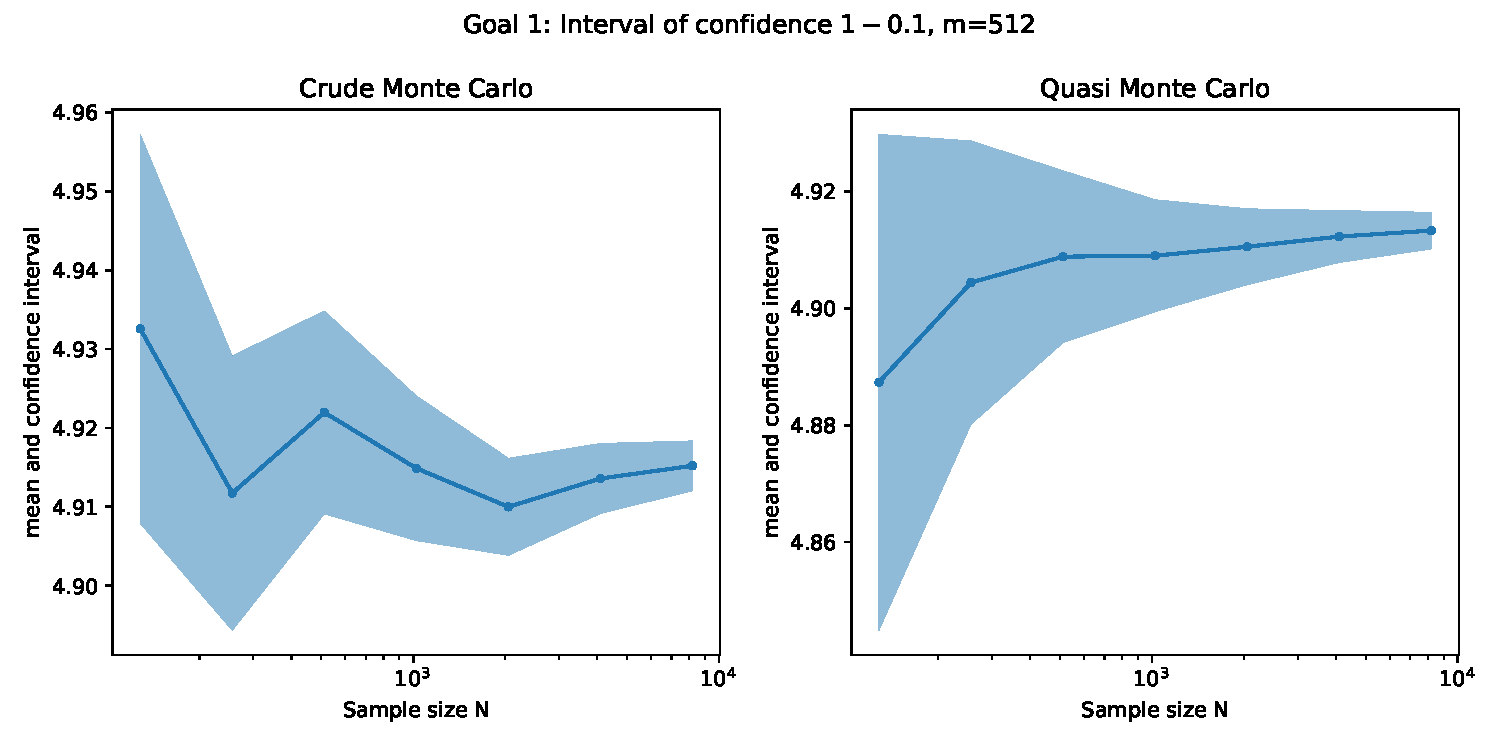
\includegraphics[width=\textwidth]{graphics/q1error.pdf}}
    \caption{Evolution of the error (standard deviation) given by (Q)MC with respect to the sample size}
    \label{fig:q1error}
\end{figure}
We see that like the theory predicted, the MC method has a convergence of order $1/\sqrt{N}$. The factor become smaller as the dimension $m$ gets bigger. This is because $m$ is the discretization of the Wiener process, which is better for higher values. For the QMC method we see that we do not obtain a better convergence, due to the non-smoothness of the integrant.
\part{}
%Implement now the pre-integration trick. First, generate randomized (Q)MC points over ${[0,1]}^{m−1}$, and decide on which direction $xj$ to perform the integration and discuss your choice (or, alternatively, compare numerically different choices) depending also on the adopted re-parametrization of the Brownian path. Use the pre-integration approach to estimate Vi using both QMC and MC. Estimate your (Q)Monte Carlo error using sample sizes $N = 27,...,213$. Plot the estimated error versus N. Compare your results to those obtained in point 1 in terms of error and computational cost.
A point that is important in the implementation of the pre-integration trick, is to have a good estimation of the value of the integral. Only likewise we will have a regular integrant for the QMC method and supposedly obtain a better convergence. If we first have a good approximation of the support of $\phi(.,x_{-j})$, the integral can be done on a interval where the function is actually smooth, and a quadrature will be precise. The implementation we choose in \prettyref{eq:trans} do not have a simple expression with respect to all variables. When the index is even, the variable appear in expressions like $\sqrt{-2\log{U_{2k}}}$ and when odd in expressions like $(\cos,\sin)(2\pi U_{2k-1})$. The first one is decreasing and the the second is not. Moreover if we take off the first two terms of the sum in $W_i$ we have 
$$W_i(U)
= \sum_{k=1}^i \sqrt{t_k-t_{k-1}}Z_k(U)
= \sqrt{t_1} \sqrt{-2\log{U_{2}}}(\cos+\sin)(2\pi U_{1})
+ \sum_{k=3}^i \sqrt{t_k-t_{k-1}}Z_k(U),$$
where the rest of the sum does not imply a variable with index one or two. We then see that $W$ must be monotone with respect to the second variable. Actually this argument is valid for any variable with even index. Now since $\phi(U)= \frac{1}{m}\sum_{i=1} ^m S_i\big(W_i(U)\big) - K$ it is suffisient to show that $S_i$ is increasing. We have indeed that $S_i(W_i) = S_0 e^{(r-\s^2/2)t_i + \s W_i}$ is increasing, assuring that $\phi(U)$ is monotone, as we wanted.
The function $\phi$ has then at most one root in $[0,1]$.

In our implementation, the variables are in a different permutation for the transformation of the uniform variable into the Gaussian one: instead of alternating the pairs, the vector is cut in two halves that are being transformed into the angle and the radius variable. However, the second variable is a fixed point of this permutation, so we can keep the second variable for the pre-integration.
\begin{figure}[H] 
    \centering{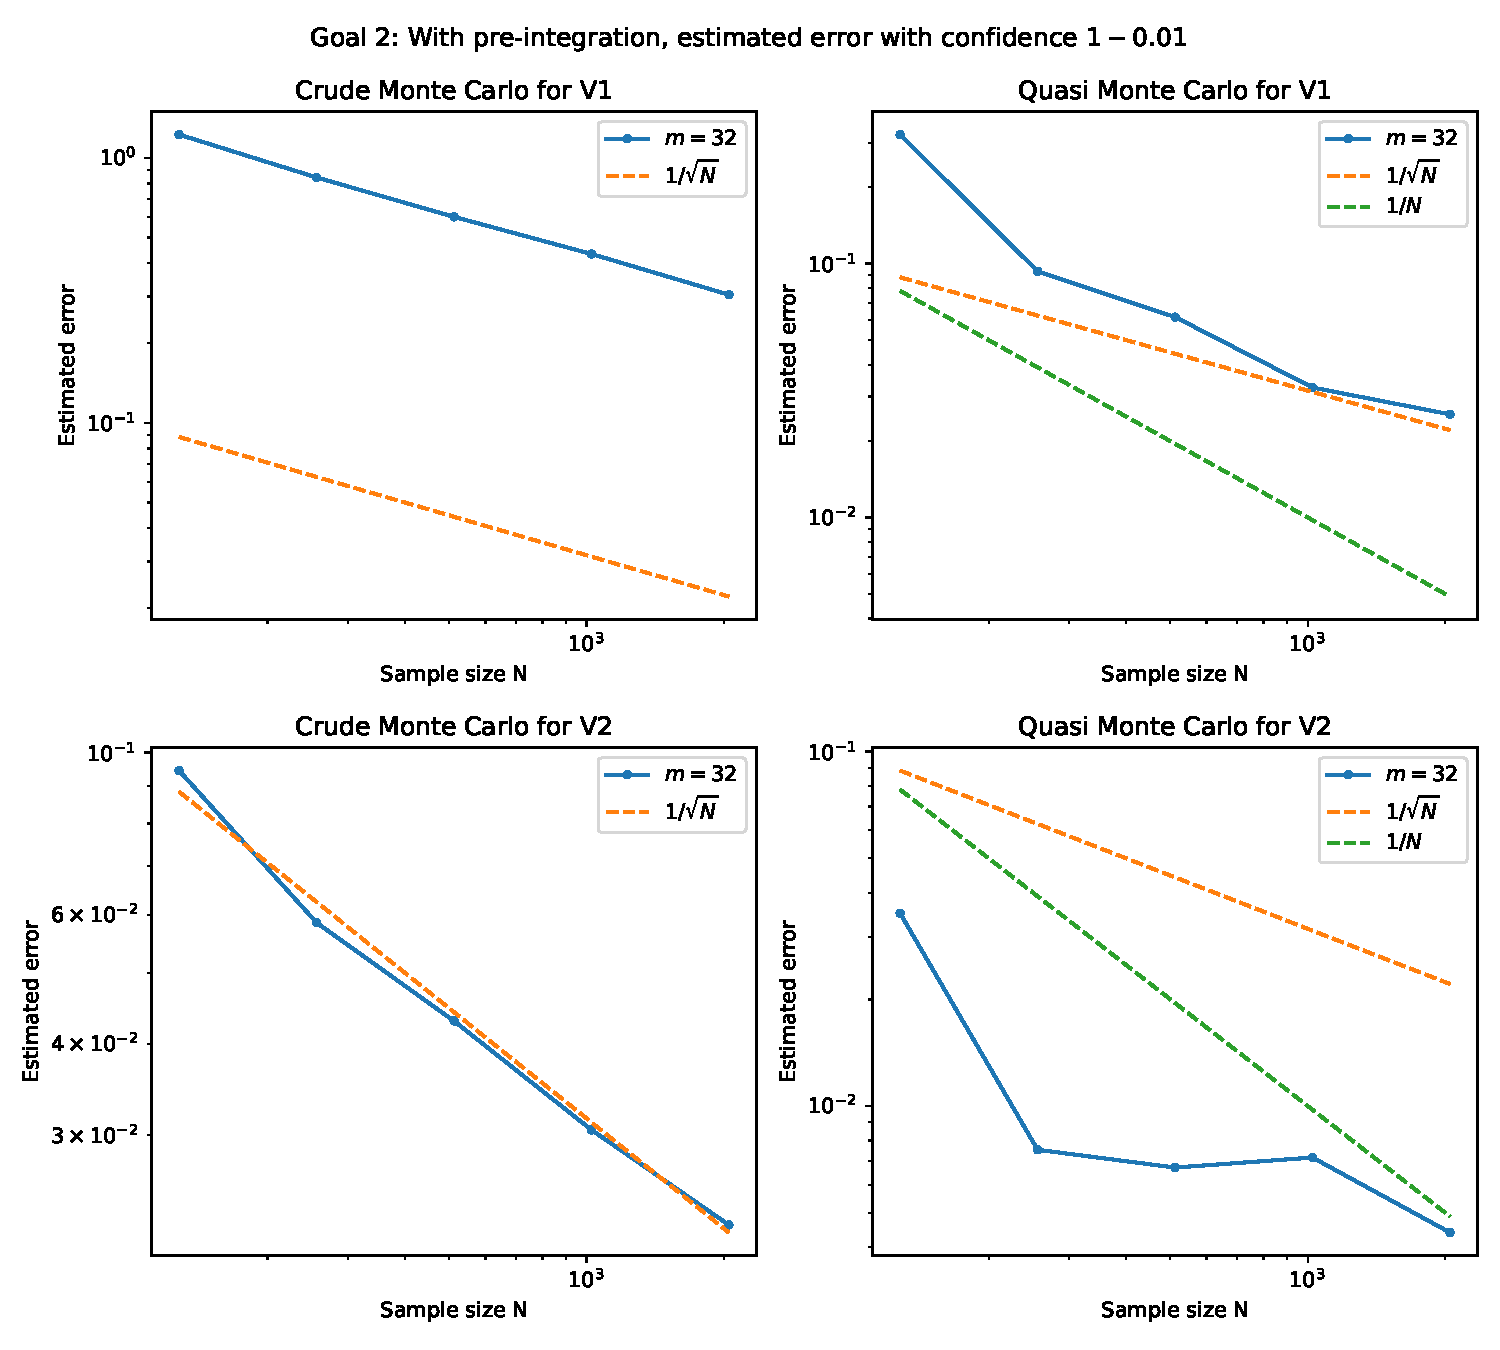
\includegraphics[width=\textwidth]{graphics/q2error.pdf}}
    \caption{With re-integration: evolution of the error (standard deviation) given by (Q)MC with respect to the sample size}
    \label{fig:q2error}
\end{figure}
\begin{figure}[H] 
    \centering{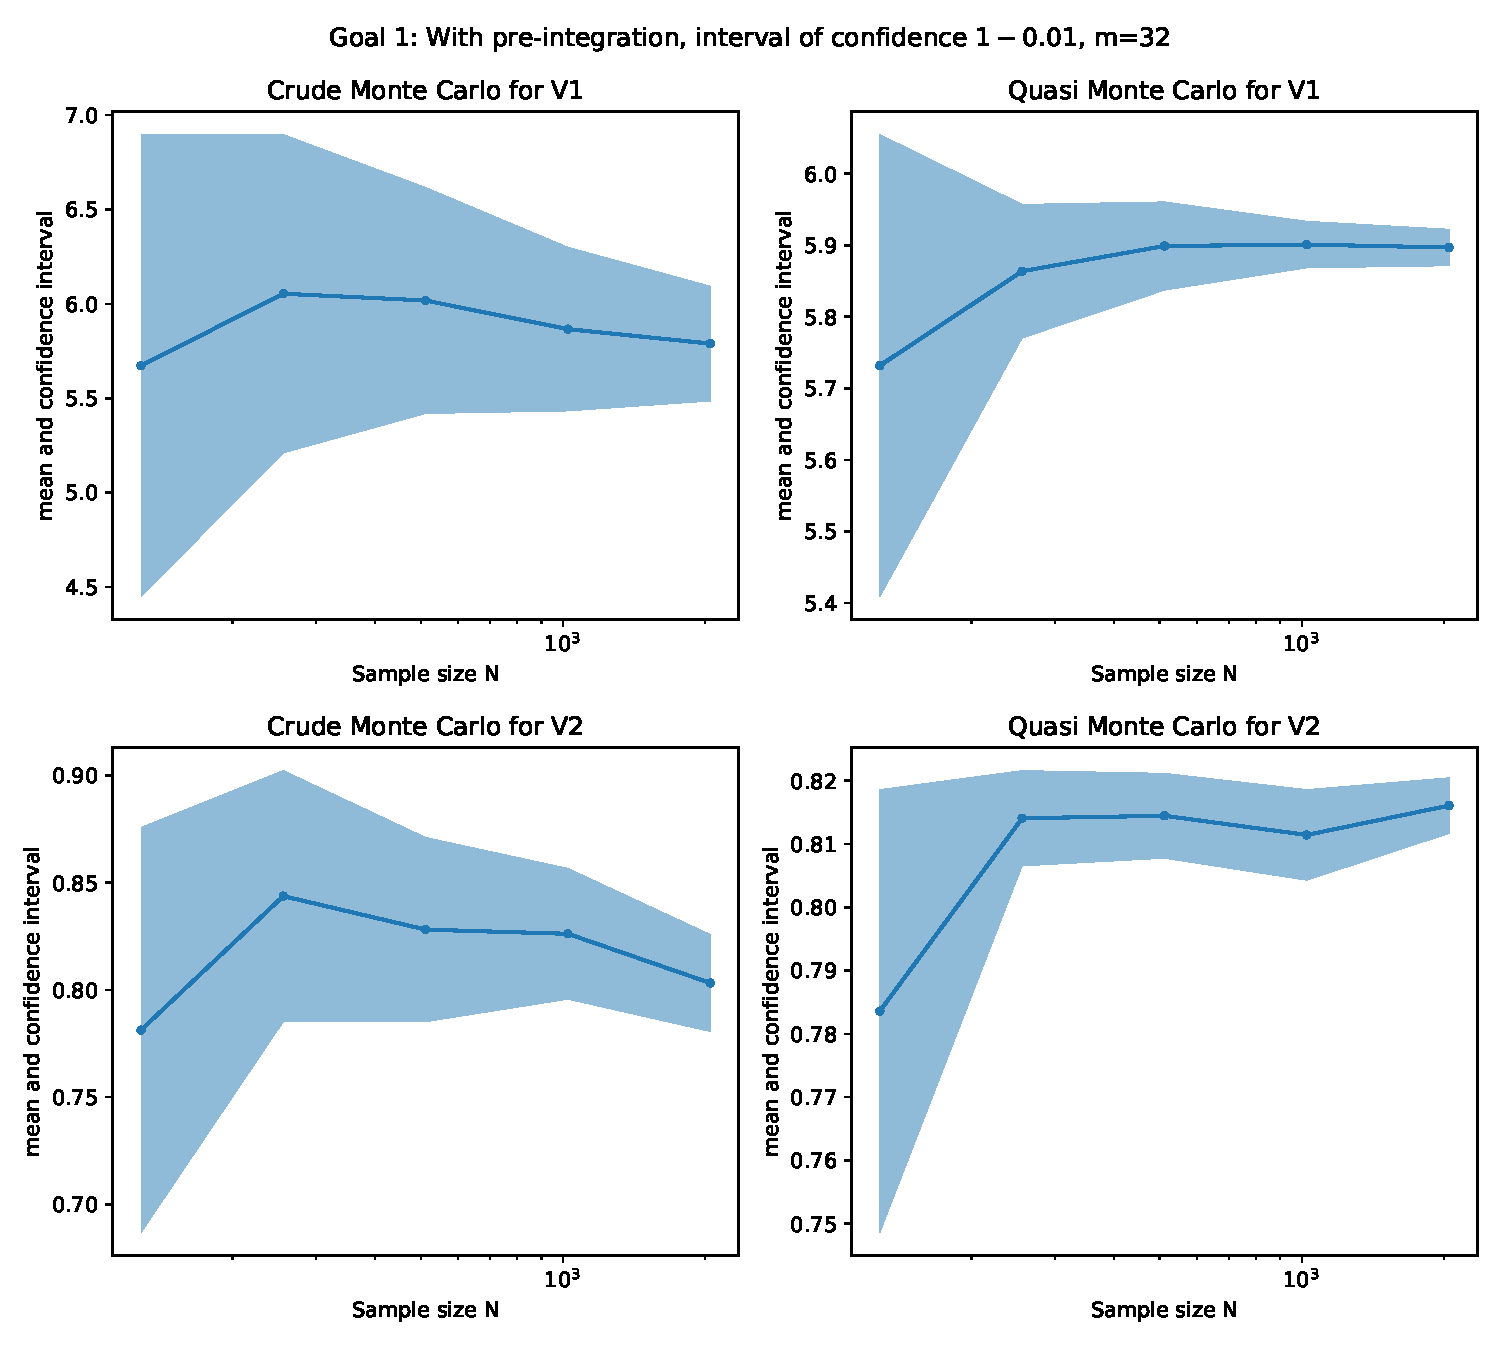
\includegraphics[width=\textwidth]{graphics/q2interval.pdf}}
    \caption{With preintegration: evolution of the mean and the interval given by (Q)MC with respect to the sample size}
    \label{fig:q2interval}
\end{figure}
\part{}
Based on a previous run made with sample size $\tilde{N}$, the supposed sample size we should use is
$$N=\frac{c_{1-\alpha}^2\hat{\sigma}^2_{\tilde{N}}}{\text{tol}^2} = \frac{\text{err}^2\tilde{N}}{\text{tol}^2}
= \frac{\text{err}^2\tilde{N}}{10^{-4}\hat{\mu}_{\tilde{N}}^2}$$ 
(with the condition that the first run is big enough to be meaningful) and where $\text{tol}=10^{-2}\hat{\mu}_{\tilde{N}}$.

When $K=500$, it is really greater than the mean of $S$, $S_0e^{rT}$. As a result, most of the the mass of $S$ falls in the region where $/Psi=0$. Hence a crude Monte Carlo estimator will be very ineffective as only few replicas of $S$ will fall in the “interesting” region $S > K$. The idea would then be to “artificially” push the distribution to the right. This method is the importance sampling. This can be achieved, for instance, by increasing the drift parameter $r$ in the dynamics of $S$. The new parameter is $\tilde{r}$ and its associated new variable $\tilde{S}$ with likelihood ration in the importance sampling estimator reads by a formula of the course: 
$$\exp\Big(\frac{\tilde{r}-r}{\sigma}\big(\frac{T(\tilde{r}-r)}{2\sigma}+\tilde{w_T}\big)\Big)$$
The 

%Consider now $K = 500$ and the goal of computing V1 and V2 with given relative accuracy $10^{−2}$ in the mean squared sense. What sample size should be used for a crude MC estimator? Propose a variance reduction technique to improve the performance of the crude MC estimator.
\part{}
%Repeat point 3 for the QMC estimator (with and without the pre-integration trick). What do you observe? Can the variance reduction technique proposed in point 3 be used also in this context? If yes, how?

\appendix
\section{mes\_statsp.y}
\python{mes_stats.py}
\section{Payoff.py}
\python{Payoff.py}
\section{q1.py}
\python{q1.py}
\section{q2.py}
\python{q2.py}
\section{q3.py}
%\python{q3.py}

\end{document}